\section{Anhang} \label{Anhang}
\subsection{Metadaten der LUBW Fachsysteme} \label{Metadaten der LUBW Fachsysteme}
In den folgenden Abschnitten sind die Metadaten und Relationen der Untersuchten Dokumente in \ac{FADO} abgebildet.
\subsubsection{Metadaten des Fachsystems FADO / Urteile}
\begin{table}[ht]
\begin{center}
\begin{tabular}{|l|l|}
\hline
\textbf{Metadaten:} & \textbf{Werte:} \\ \hline
Fachsystem & Vorgabe \\ \hline
ID & Generiert \\ \hline
Titel & Freitext \\ \hline
Tenor & Freitext \\ \hline
Kommentar & Freitext \\ \hline
Orientierungssatz & Freitext \\ \hline
Norm & Freitext \\ \hline
Leitsatz & Freitext \\ \hline
Gericht & Freitext \\ \hline
Entscheidungsform & Freitext \\ \hline
Entscheidungsdatum & Datum \\ \hline
Aktenzeichen & Freitext \\ \hline
Vorgericht & Freitext \\ \hline
Nachgericht & Freitext \\ \hline
Sachverhalt & Freitext \\ \hline
Gr�nde & Freitext \\ \hline
Unsichtbar & Bool \\ \hline
ausblenden & Bool \\ \hline
\end{tabular}
\label{Metadaten der Urteile in FADO}
\caption{Metadaten der Urteile in FADO}
\end{center}
\end{table}

\begin{table}[ht]
\begin{center}
\begin{tabular}{|l|l|}
\hline
\textbf{Relationen:} & \textbf{Werte:} \\ \hline
Thema & Vorgabe \\ \hline
geh�rt zu Fachobjekt & Vorgabe \\ \hline
hat Schlagwort & Vorgabe \\ \hline
ist vom Typ & Vorgabe \\ \hline
enthalten in Fachsystem & Vorgabe \\ \hline
wird referenziert von & Vorgabe \\ \hline
\end{tabular}
\label{Relationen der Urteile in FADO}
\caption{Relationen der Urteile in FADO}
\end{center}
\end{table}

\newpage
\subsubsection{Metadaten des Fachsystems FADO / Forschungsvorhaben}

\begin{table}[!ht]
\begin{center}
\begin{tabular}{|l|l|}
\hline
\textbf{Metadaten:} & \textbf{Werte:} \\ \hline
Fachsystem & Vorgabe \\ \hline
ID & Generiert \\ \hline
Title & Freitext \\ \hline
Kurzbeschreibung & Freitext \\ \hline
Kommentar & Freitext \\ \hline
F�rderbereich & Freitext \\ \hline
Beginn & Datum \\ \hline
Ende & Datum \\ \hline
Projektnummer & Freitext \\ \hline
F�rderkennzeichen & Freitext \\ \hline
Unsichtbar & Bool \\ \hline
ausblenden & Bool \\ \hline
\end{tabular}
\label{Metadaten der Forschungsvorhaben in FADO}
\caption{Metadaten der Forschungsvorhaben in FADO}
\end{center}
\end{table}

\begin{table}[!ht]
\begin{center}
\begin{tabular}{|l|l|}
\hline
\textbf{Relationen:} & \textbf{Werte:} \\ \hline
Thema & Vorgabe \\ \hline
geh�rt zu Fachobjekt & Vorgabe \\ \hline
hat Abschlussbericht & Vorgabe \\ \hline
hat Forschungsberichtsblatt & Vorgabe \\ \hline
hat Projektskizze & Vorgabe \\ \hline
hat Schlagwort & Vorgabe \\ \hline
hat Zwischenbericht & Vorgabe \\ \hline
wird geleitet von & Vorgabe \\ \hline
wird referenziert von & Vorgabe \\ \hline
\end{tabular}
\label{Relationen der Forschungsvorhaben in FADO}
\caption{Relationen der Forschungsvorhaben in FADO}
\end{center}
\end{table}

\newpage
\subsubsection{Metadaten des Fachsystems FADO / Berichte}

\begin{table}[!ht]
\begin{center}
\begin{tabular}{|l|l|}
\hline
\textbf{Metadaten:} & \textbf{Werte:} \\ \hline
Fachsystem & Vorgabe \\ \hline
ID & Generiert \\ \hline
Titel & Freitext \\ \hline
Kurzbeschreibung & Freitext \\ \hline
Kommentar & Freitext \\ \hline
Kurztitel & Freitext \\ \hline
Untertitel & Freitext \\ \hline
Fachthema & Freitext \\ \hline
Herausgeber & Freitext \\ \hline
Redaktion & Freitext \\ \hline
Version & Freitext \\ \hline
Stand & Datum \\ \hline
Seitenzahl & Freitext \\ \hline
Seite (von-bis) & Freitext \\ \hline
Reihe & Freitext \\ \hline
Bandnummer & Freitext \\ \hline
ISSN & Freitext \\ \hline
ISBN & Freitext \\ \hline
Preis & Freitext \\ \hline
Medium & Freitext \\ \hline
Shoprelevant & Bool \\ \hline
Shoplink & URL \\ \hline
HTML-Datei & Data \\ \hline
PDF-Datei & Data \\ \hline
Weitere Datei & Data \\ \hline
Format dieser Datei & Freitext \\ \hline
Unsichtbar & Bool \\ \hline
ausblenden & Bool \\ \hline
\end{tabular}
\label{Metadaten der Berichte in FADO}
\caption{Metadaten der Berichte in FADO}
\end{center}
\end{table}

\begin{table}[!ht]
\begin{center}
\begin{tabular}{|l|l|}
\hline
\textbf{Relationen:} & \textbf{Werte:} \\ \hline
betrift Thema & Vorgabe \\ \hline
geh�rt zu Fachobjekt & Vorgabe \\ \hline
hat Autor & Vorgabe \\ \hline
hat Schlagwort & Vorgabe \\ \hline
ist vom Typ & Vorgabe \\ \hline
enthalten in Fachsystem & Vorgabe \\ \hline
ist Abschlussbericht von & Vorgabe \\ \hline
ist Forschungsberichtsblatt von & Vorgabe \\ \hline
ist Projektskizze von & Vorgabe \\ \hline
ist Zwischenbericht von & Vorgabe \\ \hline
wird referenziert von & Vorgabe \\ \hline
\end{tabular}
\label{Relationen der Berichte in FADO}
\caption{Relationen der Berichte in FADO}
\end{center}
\end{table}

\newpage
\subsubsection{Metadaten des DRS} \label{Anhang Metadaten des DRS}

\begin{table}[htbp]
\begin{center}
\begin{tabular}{|l|l|}
\hline
\textbf{Metadaten:} & \textbf{Werte:} \\ \hline
G�ltigkeit & Vorgabe \\ \hline
Titel & Freitext \\ \hline
Aktenzeichen & Freitext \\ \hline
Kurz-Titel & Vorgabe \\ \hline
Dokumentart & Vorgabe \\ \hline
Herausgeber & Vorgabe \\ \hline
Erscheinungsort & Vorgabe \\ \hline
Handbuch & Vorgabe \\ \hline
Kapitel & Vorgabe \\ \hline
Fundstelle & Vorgabe \\ \hline
Fassung & Vorgabe \\ \hline
�nderung & Vorgabe \\ \hline
Gr��e & Zahl \\ \hline
Formate & Vorgabe \\ \hline
\end{tabular}
\label{Metadaten des DRS}
\caption{Metadaten des DRS}
\end{center}
\end{table}

Zu beachten ist hier, dass die Metadaten-Tags Fassung und \"Anderung zusammengesetzte Daten enthalten, wie es in der Abbildung \ref{Suchmaske DRS} zu sehen ist.

\newpage
\subsubsection{Metadaten des Bildarchivs}\label{Anhang Metadaten des Bildarchivs}

\begin{table}[htbp]
\begin{center}
\begin{tabular}{|l|l|}
\hline
\textbf{Metadaten:} & \textbf{Werte:} \\ \hline
Objektart & Freitext \\ \hline
Objektname & Freitext \\ \hline
ID & Generiert \\ \hline
URL & URL \\ \hline
Dateityp & Vorgabe \\ \hline
Name & Freitext \\ \hline
Kurzname & Freitext \\ \hline
Erstellt am & Datum \\ \hline
Autor & Freitext \\ \hline
Besitzer & Besitzer \\ \hline
Bemerkung & Freitext \\ \hline
\end{tabular}
\label{Metadaten des Bildarchivs}
\caption{Metadaten des Bildarchivs}
\end{center}
\end{table}

\newpage
\subsection{Metadaten der ICT-ENSURE} \label{Metadaten der ICT-ENSURE}
In den folgenden Abschnitten sind die Metadaten der Dokumente der \ac{ICT-ENSURE} zu finden. Diese werden hier in UML-Form abgebildet, was auch dem eigentlichen Datenmodell hinter \ac{ICT-ENSURE} entspricht. Alle Felder, die im Modell abgebildet sind, m\"ussen sp\"ater im \ac{ECM}-System Verwendung finden, mit Ausnahme der Klassen DocumentServer und URLGenerator. \cite{ICT-ENSURE_Bericht}

\begin{figure}[!ht]
\centering
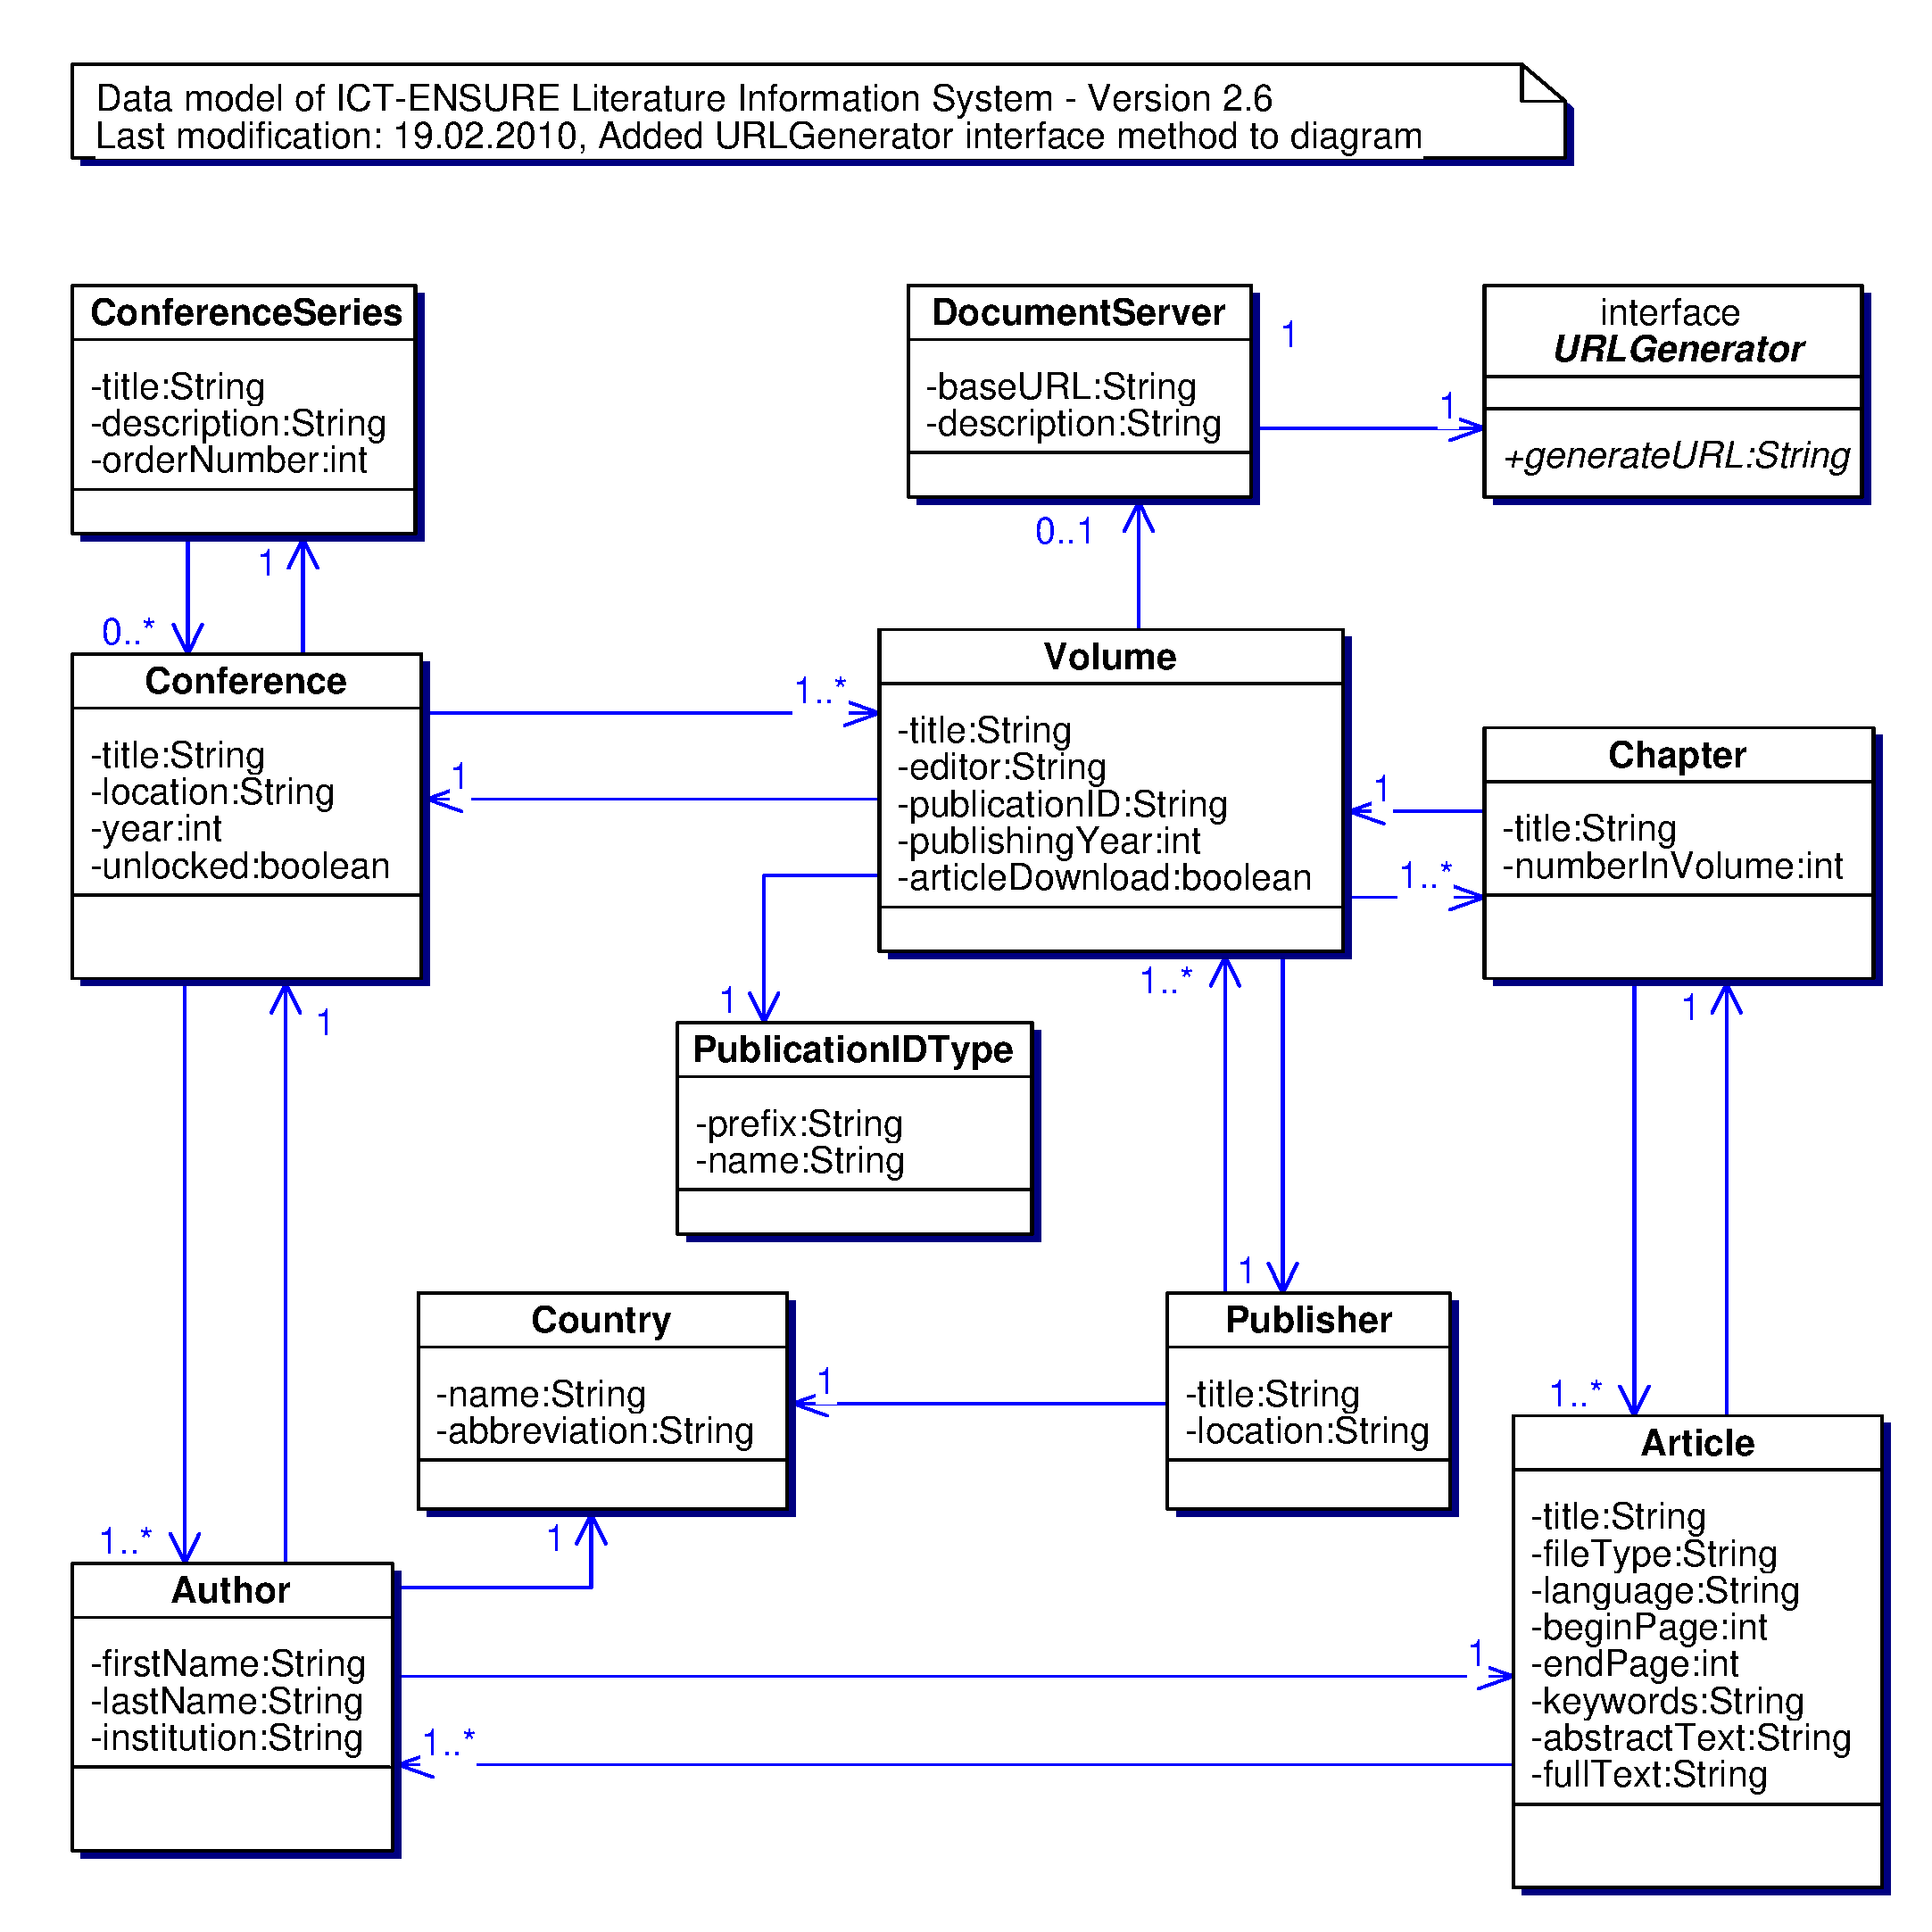
\includegraphics[width=15cm]{Bilder/Datenmodell_LitDB_V26_2010-03-11_Reduziert_fuer_Addendum.eps}
\caption{Datenmodell des Literaturarchivs \ac{ICT-ENSURE} \cite{ICT-ENSURE_Bericht}}
\label{Datenmodell ICT-ENSURE}
\centering
\end{figure}

\newpage
\subsection{Exif-Metadaten von Alfresco} \label{Exif-Metadaten von Alfresco}

\begin{figure}[!ht]
\centering
\includegraphics[width=12cm]{Bilder/Exif_Alfresco.jpg}
\caption{Ausgelesene Exif-Daten von Alfresco}
\label{Exif-Datein von Alfresco}
\centering
\end{figure}


% \FloatBarrier
\newpage
\subsection{Bilder des Datenmodells} \label{Bilder des Datenmodells} 

\begin{figure}[!ht]
\centering
\includegraphics[width=4.7cm]{Bilder/Datenmodell/Package-Standard-Metadaten90.jpg}
\caption{Package Standard Metadaten}
\label{Package Standard Metadaten Rotated}
\centering
\end{figure}

\begin{figure}[!ht]
\centering
\includegraphics[width=4.2cm]{Bilder/Datenmodell/Package-Abstrakte-Metadaten-Teil1_90.jpg}
\caption{Package Abstrakte Standard Metadaten Teil 1 \ac{INSPIRE}}
\label{Package Abstrakte Standard Metadaten Teil 1 Rotated}
\centering
\end{figure}

\FloatBarrier
\subsection{Darstellung der Metadaten in Alfresco}\label{Metadaten in der Alfrescooberfl\"ache}
\begin{figure}[!ht]
\centering
\includegraphics[width=11cm]{Bilder/Alfresco_Metadatendarstellung.jpg}
\caption{Darstellung der Metadaten in der Dokumenten\"ubersicht}
\label{h}
\centering
\end{figure}

\newpage
\subsection{Darstellung einer Bulk-Import XML-Datei}\label{Darstellung einer Bulk-Import XML-Datei}
\lstinputlisting[language=html, caption=Darstellung einer XML-Datei f\"ur den Bulk-Import]{Code/bulk-import.xml}

\newpage
\subsection{Repositorydarstellung in Liferay}\label{Repositorydarstellung in Liferay}
\begin{figure}[!ht]
\centering
\includegraphics[width=10cm]{Bilder/Liferay-Repo.jpg}
\caption{Das Textfeld Gr\"unde nach der Bearbeitung}
\label{Repositorydarstellung in Liferay Bild}
\centering
\end{figure}


% \newpage
\subsection{Die Methode createCmisSession()}\label{Methode createCmisSession}
\lstinputlisting[language=java, caption=Die Methode createCmisSession()]{Code/createCmisSession.java}